\section{Используемые технологии}

Оптимизируемое приложение является текстовым редактором с возможностью проверки орфографии, следовательно, критические мета могут присутствовать как в пользовательском интерфейсе (frontend), такие как, например, повторная перерисовка элементов, так и в основном процессе (backend).

Таким образом, необходимо изучить технологии работы с front- и back-end приложениями и использовать лучшие практики для достижения оптимальной производительности приложения.

Технологии, использованные при оптимизации приложения, описаны ниже.

% Общие технологии разработки
\subsection{Общие технологии разработки}

Общими технологиями при разработке frontend и backend является Javascript, Typescript, npm и Webpack.

% Javascript
\subsubsection{Javascript}

Javascript (JS) - это легковесный интерпретируемый динамический язык программирования, который применяется при разработке сценариев веб-страниц, которые обеспечивают интерактивность сайтам, и при разработке серверных или кроссплатформенных настольных приложений. Является одной из реализаций спецификации ECMAScript.



% Typescript
\subsubsection{Typescript}

Typescript (TS) - это строго типизированный и компилируемый язык, основанный на Javascript~\cite{TS}. Код, написанный на Typescript, компилируется в Javascript-код, что позволяет использовать TS везде, где используется JS.

С помощью TS разрабатывать поддерживать, масштабировать и тестировать сложные комплексные программы можно быстрее и проще, чем на JS, так как ещё на моменте разработки компилятор будет указывать на фрагменты кода, где допущена ошибка, что практически исключает вероятность возникновения ошибки при работе программы.

Typescript исключает возможность неправильной реализации или некорректного вызова методов и заставляет разработчика продумать логику приложения (например, на уровне методов) до самой реализации~\cite{TS}.

% npm
\subsubsection{npm}

npm - это менеджер пакетов, позволяющий разработчикам обмениваться инструментами, устанавливать различные модули и управлять их зависимостями~\cite{npm}.

npm предоставляет возможность добавлять в свои проекты пакеты кода, а так же делиться своими, что избавляет от повторного написания больших объемов кода; создавать общую базу кода при командной разработке; управлять зависимостями проектов.

% Webpack
\subsubsection{Webpack}
Webpack - это инструмент для сборки модулей. Он может анализировать приложение, создавать его граф зависимостей и собирать приложение в виде бандлов (совокупностей программных данных, объединённых по какому-либо признаку), на которые приложение будет ссылаться при выполнении.

Обычно при разработке приложения, не важно, frontend или backend, код разделяется на несколько частей (модулей), обеспечивающих специфичные методы обработки данных. Но это может повлечь множество проблем при разработке и выполнении программы, таких как, например, разработчик может забыть подключить какие-либо скрипт или расположить их в неправильном порядке. Например, если вызывать скрипт, в котором используется какой-либо фреймворк до того, как он был загружен, приложение будет выполняться неправильно.

Webpack позволяет избежать подобные ситуации и берёт сборку приложения на себя.

Сборка приложения включает в себя создание бандлов приложения, подключение необходимых зависимостей, преобразование кода к минифицированному и другие этапы. Все эти этапы разработчик может указать в отдельном файле конфигурации и использовать при сборке.

В общем виде, работа Webpack показана на рисунке~\ref{img:webpack}

\begin{figure}[H]
  \centering
  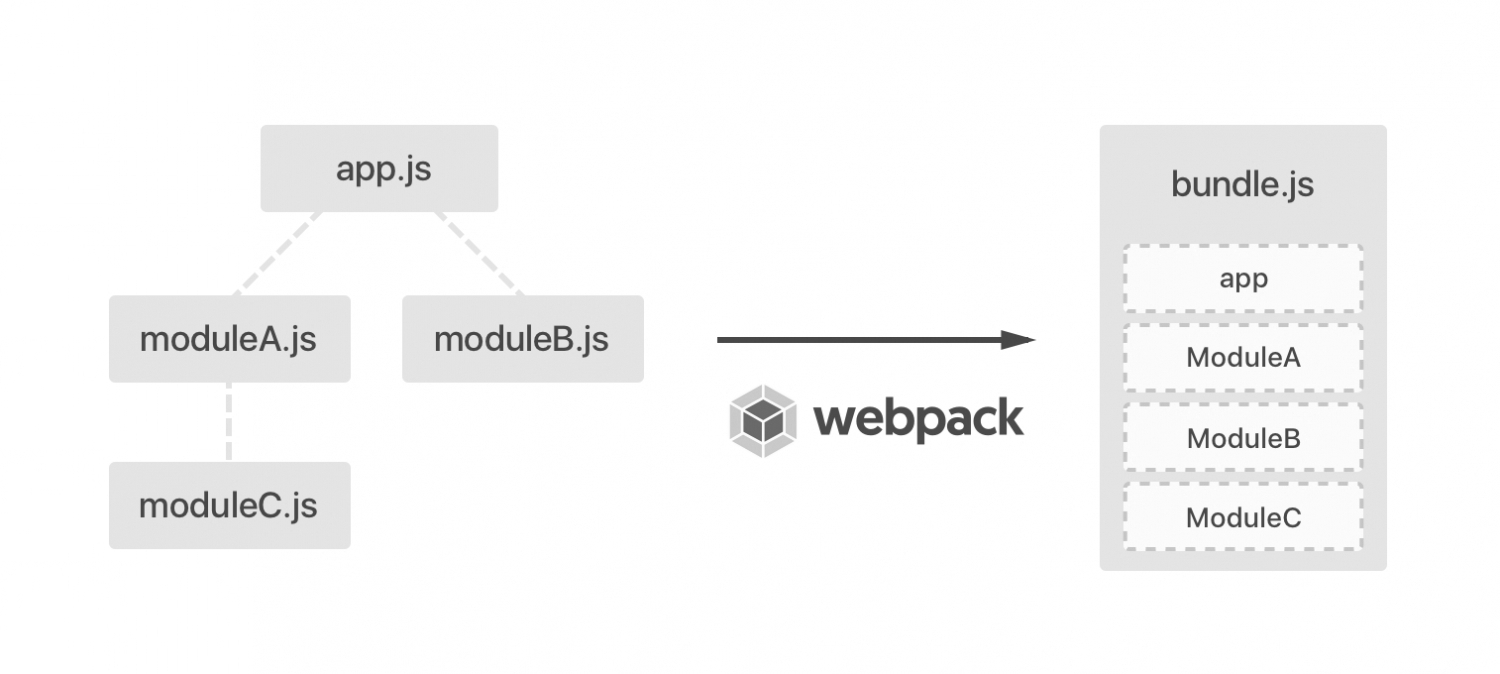
\includegraphics[width=0.95\textwidth]{assets/images/theoretical/webpack.jpg}
  \caption{Работа Webpack}
  \label{img:webpack}
\end{figure}


% Frontend
\subsection{Frontend}

При разработке frontend были также использованы HTML, CSS и React.

% HTML
\subsubsection{HTML}

HTML (HyperText Markup Language - ``Язык гипертекстовой разметки'') - это стандартизированный язык разметки документов, определяющий содержание и структуру веб-контента.

Веб-браузер может интерпретировать описанный с помощью HTML документ и отобразить его структуру на экране пользователя.

При загрузке HTML браузером, создаётся объектная модель документа~-~DOM. DOM - это стандартная объектная модель программного интерфейса HTML, которая определяет:

\begin{itemize}
  \item Элементы HTML как объекты;
  \item Свойства всех HTML элементов;
  \item Методы доступа ко всем HTML элементам;
  \item События для всех HTML элементов.
\end{itemize}

Другими словами, DOM - это стандарт того, как можно получить, изменить, добавить или удалить HTML элементы.

Благодаря DOM можно описать все элементы как набор утверждений и формул, изменение которых ведёт к автоматическому перерасчёту всех зависимостей, и, таким образом, сделать сайт реактивным, т.е. способным обновляться при изменении внутреннего состояния, с помощью, например, JS.

Реактивность реализована во многих frontend-фреймворках и библиотеках. Я выбрал React, так как он даёт более высокий уровень гибкости при разработке.

% CSS
\subsubsection{CSS}

CSS (Cascading Style Sheets - ``каскадные таблицы стилей'') язык описания форматирования документа, написанного с помощью языка разметки~\cite{CSS}. Обычно с помощью css описывают оформление веб-страниц, написанных с помощью HTML.

CSS используется для задания расположения отдельных элементов, используемых шрифтов, цветов, анимаций и других параметров внешнего вида страницы.

CSS поддерживает таблицы стилей для конкретных носителей, поэтому разработчик может адаптировать представление своих документов к браузерам, скринридерам и другим устройствам.

Каскадные таблицы описывают правила форматирования элементов с помощью свойств и указания доступных значений этих свойств. К каждому элементу можно добавить определённый ограниченный набор свойств, в то время как другие свойства не будут оказывать на элемент никакого влияния~\cite{CSS}.

% React
\subsubsection{React}

React - это библиотека для создания пользовательских интерфейсов~\cite{React}. React используется для визуализации и в связке с другими библиотеками. Например, React Native можно использовать при разработке мобильных приложений, а с помощью React 360 - при разработке приложений виртуальной реальности.

При создании веб-приложений, используется связка React и ReactDOM. При этом создаются React-элементы, которые нужно вывести на страницу, а ReactDOM обновляет DOM, чтобы он соответствовал переданным в него React-элементам.

Основная цель React - минимизация ошибок при разработке пользовательских интерфейсов~\cite{React}. Это достигается за счёт использования автономных логических фрагментов кода - компонентов, которые описывают определённую часть пользовательского интерфейса. Полученные компоненты можно объединить в комплексный объект и создать полноценный пользовательский интерфейс.

React предоставляет удобный интерфейс для разработки элементов страницы - JSX.

Каждый JSX-элемент - это расширение JS, которое позволяет максимально понятно описывать внешний вид элемента, при этом включая в себя все преимущества JS. С помощью JSX можно описать DOM-элемент используя не строки, а Javascript, React-элементы, которые затем встраиваются в DOM страницы~\cite{React}. Пример JSX-компонента представлен в листинге~\ref{lst:jsx}.

\begin{lstlisting}[style=ES6, caption={Пример JSX-элемента}, label = {lst:jsx}]
  const element = <h1>Hello, world!</h1>;
\end{lstlisting}

\subsection{Backend}

При разработке backend также были использованы Node.js и Electron.

% Node
\subsubsection{Node.js}

Node.js представляет собой среду выполнения Javascript-кода, вне браузера. Node.js основан на движке Javascript V8, который позволяет транслировать JS-код в машинный код. Прежде всего, Node.js предназначен для создания серверных и настольных приложений.

Одним из преимуществ Node.js является то, что если разработчик владеет навыками написания frontend Javascript кода, то он без проблем сможет разработать backend код, и благодаря этому он является одним из популярных языков написания серверных приложений.

Так же одним из достоинств языка является наличие механизма асинхронного ввода-вывода, а именно использование неблокирующих операций ввода-вывода. Это значит, что главный поток не будет блокироваться операциями ввода-вывода и сервер будет продолжать обрабатывать запросы. Это возможно из-за того, что в V8, а, следовательно, Node.js, используется цикл событий, который ожидает прибытия и проводит рассылку событий и выполняет операции только когда произошло определённое событие.



% Electron
\subsubsection{Electron}

Electron - это фреймворк для разработки настольных кроссплатформенных приложений с использованием JS, HTML и CSS~\cite{electron}.

В основе Electron лежат проекты Chromium и Node.js, объединённые в единую среду, обеспечивающую выполнение приложения. Ввиду этого Electron наследует все преимущества этих двух проектов:

\begin{itemize}
  \item Chromium предоставляет современный механизм рендера HTML-страниц, способы обработки событий, средства разработчика и т.д.;
  \item Node.js предоставляет возможность работы с файловой системой пользователя, высокую скорость выполнения операций и возможность использования модулей;
  \item Оба этих проекта предоставляют возможность использования движка V8, который, в свою очередь, позволяет использовать последние версии спецификации ECMAScript.
\end{itemize}

Приложение Electron представляет собой окно браузера, в котором открыто единственное окно - ваше приложение.